% % % % % % % % % % % % % % % % % % % % % % % % % % % % % % % % % %
%\documentclass[runningheads]{llncs}
%\documentclass[12pt,letterpaper]{article}
%\documentclass[preprint,12pt]{elsarticle}
%\documentclass{sig-alternate}
\documentclass[10pt,preprint]{sigplanconf}

% https://avandeursen.com/2013/07/10/research-paper-writing-recommendations/


% packages
\usepackage{xspace}
\usepackage{ifthen}
\usepackage{amsbsy}
\usepackage{amssymb}
\usepackage{balance}
\usepackage{alltt} 
\usepackage{booktabs}
\usepackage{graphicx}
\usepackage{multirow}
\usepackage{needspace}
\usepackage{microtype}
\usepackage{bold-extra}
\usepackage{subfig}
\usepackage{wrapfig}
\usepackage{balance}
\usepackage[colorlinks]{hyperref}
\usepackage[all]{hypcap}
\usepackage{xcolor}
\usepackage{textcomp}
\usepackage{listings}
\definecolor{source}{gray}{0.9}
\setcounter{tocdepth}{2}

\def\chapterautorefname{Chapter}
\def\appendixautorefname{Appendix}
\def\sectionautorefname{Section}
\def\subsectionautorefname{Section}
\def\figureautorefname{Figure}
\def\tableautorefname{Table}
\def\listingautorefname{Listing}

\lstset{
	language={},
	% characters
	tabsize=3,
	upquote=true,
	escapechar={!},
	keepspaces=true,
	breaklines=true,
	alsoletter={\#:},
	breakautoindent=true,
	columns=fullflexible,
	showstringspaces=false,
	basicstyle=\footnotesize\sffamily,
	% background
	frame=single,
    framerule=0pt,
	backgroundcolor=\color{source},
	% numbering
	numbersep=5pt,
	numberstyle=\tiny,
	numberfirstline=true,
	% captioning
	captionpos=b,
	% formatting (html)
	moredelim=[is][\textbf]{<b>}{</b>},
	moredelim=[is][\textit]{<i>}{</i>},
	moredelim=[is][\color{red}\uwave]{<u>}{</u>},
	moredelim=[is][\color{red}\sout]{<del>}{</del>},
	moredelim=[is][\color{blue}\underline]{<ins>}{</ins>}}
\newcommand{\ct}{\lstinline[backgroundcolor=\color{white},basicstyle=\footnotesize\ttfamily]}
\newcommand{\lct}[1]{{\small\tt #1}}

% proof-reading
\usepackage{xcolor}
\usepackage[normalem]{ulem}
\newcommand{\ra}{$\rightarrow$}
\newcommand{\ugh}[1]{\textcolor{red}{\uwave{#1}}} % please rephrase
\newcommand{\ins}[1]{\textcolor{blue}{\uline{#1}}} % please insert
\newcommand{\del}[1]{\textcolor{red}{\sout{#1}}} % please delete
\newcommand{\chg}[2]{\textcolor{red}{\sout{#1}}{\ra}\textcolor{blue}{\uline{#2}}} % please change
\newcommand{\chk}[1]{\textcolor{ForestGreen}{#1}} % changed, please check

% comments \nb{label}{color}{text}
\newboolean{showcomments}
\setboolean{showcomments}{true}
\ifthenelse{\boolean{showcomments}}
	{\newcommand{\nb}[3]{
		{\colorbox{#2}{\bfseries\sffamily\scriptsize\textcolor{white}{#1}}}
		{\textcolor{#2}{\sf\small$\blacktriangleright$\textit{#3}$\blacktriangleleft$}}}
	 \newcommand{\version}{\emph{\scriptsize$-$Id$-$}}}
	{\newcommand{\nb}[3]{}
	 \newcommand{\version}{}}
\newcommand{\rev}[2]{\nb{Reviewer #1}{red}{#2}}
\newcommand{\ab}[1]{\nb{Alexandre}{blue}{#1}}
\newcommand{\lr}[1]{\nb{Lukas}{pink}{#1}}
\newcommand{\ai}[1]{\nb{Alejandro}{orange}{#1}}
\newcommand{\on}[1]{\nb{Oscar}{olive}{#1}}


% graphics: \fig{position}{percentage-width}{filename}{caption}
\DeclareGraphicsExtensions{.png,.jpg,.pdf,.eps,.gif}
\graphicspath{{figures/}}
\newcommand{\fig}[4]{
	\begin{figure}[#1]
		\centering
		\includegraphics[width=#2\textwidth]{#3}
		\caption{\label{fig:#3}#4}
	\end{figure}}

\newcommand{\largefig}[4]{
	\begin{figure*}[#1]
		\centering
		\includegraphics[width=#2\textwidth]{#3}
		\caption{\label{fig:#3}#4}
	\end{figure*}}
	
\newcommand{\wrapfig}[5]{	
\begin{wrapfigure}{#1}{#2\textwidth}
  \begin{center}
    \includegraphics[width=#3\textwidth]{#4}
  \end{center}
  \caption{\label{fig:#4}#5}
\end{wrapfigure}}

% abbreviations
\newcommand{\ie}{\emph{i.e.,}\xspace}
\newcommand{\eg}{\emph{e.g.,}\xspace}
\newcommand{\etc}{\emph{etc.}\xspace}
\newcommand{\etal}{\emph{et al.}\xspace}

% lists
\newenvironment{bullets}[0]
	{\begin{itemize}}
	{\end{itemize}}

\newcommand{\seclabel}[1]{\label{sec:#1}}
\newcommand{\figlabel}[1]{\label{fig:#1}}
\newcommand{\tablabel}[1]{\label{tab:#1}}
\newcommand{\figref}[1]{Figure~\ref{fig:#1}}
\newcommand{\secref}[1]{Section~\ref{sec:#1}}


%Specialized macros
\pagenumbering{arabic}
\DeclareCaptionType{copyrightbox}
\newcommand{\myparagraph}[1]{\vspace{0.1cm}\noindent \textbf{\textit{#1.}}}



\balance

% constants
% \newcommand{\Title}{Toward Reducing Waste of Expandable Collections: The Pharo Case}
\newcommand{\Title}{Accurate VM profiler for the Cog VM}
%\newcommand{\Title}{The Dark Side of Expandable Collections: The Pharo Case}
\newcommand{\TitleShort}{\Title}
%\newcommand{\Authors}{~~~~}
\newcommand{\Authors}{Sophie Kaleba, Cl\'ement B\'era, Alexandre Bergel$^3$\\[2 ex]
$^3$Pleiad Lab, DCC, University of Chile}
\newcommand{\AuthorsShort}{}

\hypersetup{
	colorlinks=true,
	urlcolor=black,
	linkcolor=black,
	citecolor=black,
	plainpages=false,
	bookmarksopen=true,
	pdfauthor={\Authors},
	pdftitle={\Title}}
	
\newenvironment{code}
    {\begin{alltt}\sffamily}
    {\end{alltt}\normalsize}	
	
%\newcommand{\Authors}{Alexandre Bergel, Vanessa Pe\~na}
%\newcommand{\AuthorsShort}{A. Bergel, V. Pe\~na}

%\journal{Science of Computer Programming}

% \makeatletter
% \let\@copyrightspace\relax
% \makeatother
% 

%double spaced
%\renewcommand{\baselinestretch}{1.5}

\begin{document}

\special{papersize=8.5in,11in}
\setlength{\pdfpageheight}{\paperheight}
\setlength{\pdfpagewidth}{\paperwidth}

\conferenceinfo{OOPSLA '14}{Month d--d, 20yy, City, ST, Country}
\copyrightyear{2014}
\copyrightdata{978-1-nnnn-nnnn-n/yy/mm}
\doi{nnnnnnn.nnnnnnn}


%\begin{frontmatter}
\title{\Title}


\authorinfo{Sophie Kaleba$^1$, Cl\'ement B\'era$^1$, Alexandre Bergel$^2$}
           {$^1$INRIA- Lille Nord Europe, France\\
             $^2$Pleiad Lab, DCC, University of Chile, Santiago, Chile}
           {}
%\author{\Authors
%}


%\institute{~~}
%\institute{Pleiad Lab, University of Chile}
\maketitle

\begin{abstract}

%context
Code profiling enables a user to know where in an application or function the execution time is spent. The Pharo ecosystem offers several code profilers. However, most of the publicly available profilers (MessageTally, Spy, GadgetProfiler) largely ignore the activity carried out by the Pharo virtual machine, thus incurring inaccuracy in the gathered information and missing important information, such as the JIT activity.

This paper motivates and describes VMProfiler, a code execution profiler hooked into the virtual machine. VMProfiler exercises its analysis by monitoring the execution of the virtual machine. This paper presents the latest innovations carried out in VMProfiler, in particular to address some limitations related to assessing the activity of native functions (resulting from a JIT operation).

%Profiling tools are already available for Smalltalk-based languages, like MessageTally, GadgetProfiler or VMProfiler. The latter, especially, by tracking down where the time is spent on the virtual machine (VM) side, can provide significant data to help tuning the VM settings for performance.
%
%%problem
%However, while this VM profiler can identify in which functions the execution time is spent, it cannot identify where in these functions the time is spent. This is getting critical as the optimisations performed by the Just-In-Time compiler (JIT) result in functions of greater size, which are then harder to profile accurately.
%
%%solution
%In this paper, we discuss this problem and then we introduce the solution proposed to keep collecting relevant profiling data, using an API that allow us to identify, for a given function, in which bytecode range the time is spent.

\end{abstract}

%\begin{keyword}
%% keywords here, in the form: keyword \sep keyword

%% MSC codes here, in the form: \MSC code \sep code
%% or \MSC[2008] code \sep code (2000 is the default)
%profiling \sep virtual machine \sep cog
%\end{keyword}




%\end{frontmatter}
%: % % % % % % % % % % % % % % % % % % % % % % % % % % % % % % % % %

\section{Introduction}

%TEMPLATE:
%
%Context
%
%Problem
%
%Known tracks for \sd{solutions}
%	here you want to show that you are not an idiot not knowing what have been around
%
%What our solution is \ct{Set} and \ct{OrderedCollection} (so that the reader knows where the paper is going)
%
%Contribution of the paper
%
%Paper structure


%context
%main challenge in general and thus for VMs : performance

\textbf{[\`a r\'e\'ecrire]} Even though the technical specs of computers get more and more impressive, performance, both in terms of execution time and XXX, remains a major goal to be pursued). \textbf{[\`a r\'e\'ecrire]}
This statement applies of course to virtualised environments and assuring the performance of the virtual machine (VM) is critical when you aim for an overall good performance. 
Thus, it is crucial to know where the time is spent in the VM during execution : indeed, it helps identifying where to tune its settings to actually get better results.

These critical informations can be collected by profiling code, to get a precise idea of the program behaviour. 
Such profiling tools are already available in Smalltalk, like MessageTally and VMProfiler : they provide statistical/graphical reports, showing the methods in which most of the execution time is spent, and how much of this time is spent in garbage collection. However, the VM profiler, unlike MessageTally, provides statistical data about the time spent in the Cog VM. Cog~\cite{Mira08a}~ is a virtual machine designed for Smalltalk, and currently used for various Smalltalk-based languages such as Pharo~\cite{Blac09a} or Squeak~\cite{Blac07a}. It features a bytecode interpreter and a JIT. It is in the code of these features that we find out where the execution time is spent.\\

% problem 
Right now, this VM profiler cannot track down precisely where the time is spent when executing the code generated by the JIT. It can track down in which methods the time is spent, but it cannot track down in which part of those methods the time is spent. For example, assume there is a frequently used method with multiple loops. The VM profiler can tell us that most of the time is spent in this method (it is indeed frequently used), but it cannot tell in which loop the time is spent.

This problem is more and more significant as new optimisations are added to the JIT, based on the work of H\"olzle and Ungar~\cite{Holz94a}. The development branch of the JIT now features speculative inlining. In this context, the JIT generates a single machine code method for multiple bytecode methods (the method optimised and the inlined methods). The VM profiler shows that most of the time is spent in optimised code, but it is currently not possible to know in which inlined method most of the time is spent. So while we get a faster and more performant VM, we lose the ability to profile it accurately.\\

%solution
To get accurate profiling data again, the VM profiler has to be enhanced to show specifically where the time is spent in a method. To do so, we use an API usually used for debugging, that maps machine code program counter (pc) to bytecode program counter. This way, we can tell for each method appearing in the report in which bytecode range most of the time is spent.
\textbf{[add a quick presentation of the outline]}


%: % % % % % % % % % % % % % % % % % % % % % % % % % % % % % % % % %

\section{Accurate profiling of jitted code}

This section first defines the terminology used in the paper, then describes the existing VM profiler available in the Cog VM clients such as Squeak or Pharo and lastly states the problem analysed in the rest of the paper.

\subsection{Terminology}

\paragraph{Function.} In the paper, we use the term \emph{function} to discuss about executable code, in our case, method or block closures.

\paragraph{Bytecode function.} The term \emph{bytecode function} is used to talk specifically about the compiled function in the form of bytecode, for example, instances of \ct{CompiledMethod} in the case of methods. Bytecode functions are regular objects accessible from the Squeak/Pharo runtime and are present in the heap with all other objects.

\paragraph{Native function.} We use the term \emph{native function} to discuss about the representation of a function generated by Cog's JIT, which includes the native code. Native functions are not regular objects and are allocated in a specific memory zone (called the \emph{machine code zone}), which is executable.

\subsection{Existing VM profiler}

A VM profiler has been available for almost a decade in Squeak and has been recently ported to Pharo. The VM profiler allows to track down where the time is spent in the VM when executing a specific portion of code. The VM profiler computes where the time is spent in the compiled C code of the VM, in the VM plugins and in the native functions. All the results are available as a statistical report. A typical report includes two main sections, the time spent in generated code, \ie in native functions and the time spent in the compiled C code. The time spent in the compiled C code includes the time spent in the bytecode interpreter, in the garbage collector and in the just-in-time compiler. 

%MAYBE -- memory representation of the Cog execution.

\paragraph{Implementation.} Implementation-wise, the VM profiler is a sampling profiler. When profiling is started, a separate high-priority OS thread is started and collect the instruction pointers of the VM OS thread in a large circular buffer at a cadence of 1.3GHz. Once profiling stops, a primitive method is available to gather the samples from the VM into a Bitmap. To understand to which functions the samples correspond to, the VM profiler requests:
\begin{itemize}
	\item The symbol table of the VM executable and all external plugins.
	\item A description of the native functions currently present in the machine code zone
\end{itemize}
Each function (indifferently, a native function or a C function) is represented as a function symbol (the name of the function, either the Smalltalk function name with the method class and the selector or the C function symbol), a start address and the last address. The VM profiler uses these ranges to find out in which function each sample is, as shown in \figref{fig:OriginalMapping}. Then, the profiler generates a report, either in the form of a string or through a user interface.

 \begin{figure}[!htp]
     \begin{center}
         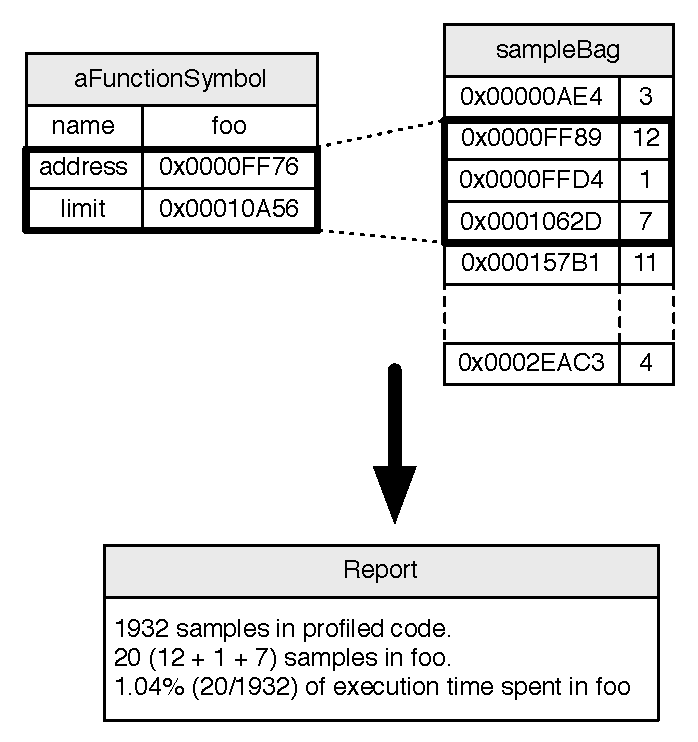
\includegraphics[width=0.9\linewidth]{OriginalMapping}
         \caption{Mapping in original code}
         \figlabel{fig:OriginalMapping}
     \end{center}
 \end{figure}
 
 
 \paragraph{Primitive Cog Constituents.}
The primitiveCollectCogCodeConstituents provides the VM profiler with the description of the native functions currently present in the machine code zone it needs. 
This primitive answers an array of pair-wise elements as shown in \figref{fig:ContentsOfCollectCogCodePrim}. The first element of the pair is the name of the native function, the second one is its starting address in the code zone.
It is called once the profiling has stopped and the samples has been gathered : the data provided by this primitive will be mapped with the samples collected.

 \begin{figure}[!htp]
     \begin{center}
         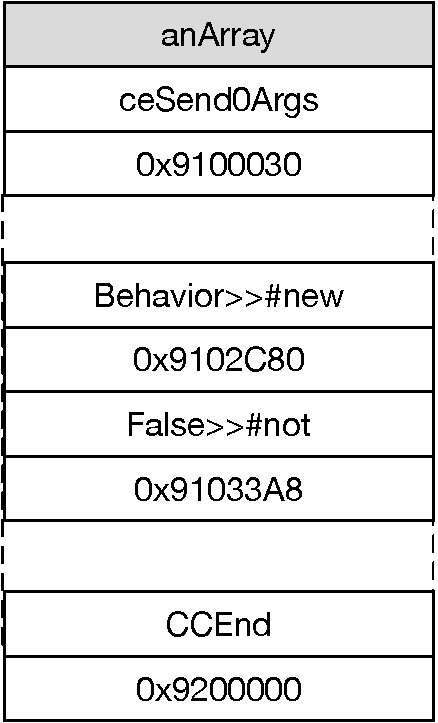
\includegraphics[width=0.4\linewidth]{ContentsOfCollectCogCodePrim}
         \caption{Cog constituents as answered by the primitive}
         \figlabel{fig:ContentsOfCollectCogCodePrim}
     \end{center}
 \end{figure}

 
\subsection{Debugger mapping}

To be able to debug native functions as if they were executed as a bytecode function by the bytecode interpreter, when Cog's JIT generates a native function for a given bytecode function, it generates a list of annotations~\cite{Ber16d} allowing to reconstruct the interpreter state of the function activation at any point where the code execution can be interrupted (message sends, conditional branch or back jumps). Each annotation includes a mapping between the pc in the machine code and the pc in the bytecode of the method. The VM is able to use these annotations to reify function activation and provide it in Squeak/Pharo.
 
\subsection{Problem statement}

The VM development team is currently working on the implementation of an optimising Just-in-time compiler for the Cog VM, with optimisations such as speculative inlining, as described in the work of H\"olzle and Ungar~\cite{Holz94a}, in a similar way to production VMs such as Java's hotspot VM\footnote{The hotspot VM is the default virtual machine for Java.}~~\cite{Pale01a} and Javascript's V8 engine\footnote{V8 is mostly used as the Javascript engine for Google Chrome and NodeJS.}~\cite{V8}. The optimising is planned as a bytecode functions to bytecode functions runtime optimising compiler, re-using the existing Just-in-time compiler as a back-end to generate native functions. In this context, optimised functions are present in the form of bytecode functions, using the extended bytecode set described in the work of B\'era \etal~\cite{Bera14a}. When profiling optimised code for benchmarks such as the Games benchmark~\cite{GameBenchs}, the VM profiler now shows that all the time is spent in a single bytecode function (the bytecode function where the rest of the functions used by the benchmark are inlined). To improve performance and tune the optimising JIT, the VM development team requires more information about where the time is spent in optimised function, for example, in which range of bytecodes the time is spent.

\emph{How to provide accurate profiling information in large native functions profiled ?}

To address this problem, we propose an implementation that take advantage of an API used for debugging, to map machine code pc to bytecode pc, to be able to identify in which bytecode range the time is spent in a function. The implementation is specific to the Cog VM, with a working version in both Squeak and Pharo. A similar design could apply in other VMs featuring similar debugging capabilities.

%: % % % % % % % % % % % % % % % % % % % % % % % % % % % % % % % % %

\section{Solution}

To profile accurately large native functions, we re-use the API available for debugging to identify in which section of the function the time is spent. The solution is split in two steps. First, we enhanced the primitive providing the description of the native functions present in the machine code zone to provide a mapping between machine code pc and bytecode pc in addition to the start address of the function. Second, we used the mapping to identify in which range of bytecodes each sample is.

\subsection{Improved primitive}

In the improved version of the primitive, if the native function has at least one machine code pc mapped to a bytecode pc, the primitive answers for the function, instead of the start address, an array starting with the start address followed by pairs of machine code pc and the corresponding mapped bytecode pc. 

+ EXAMPLE:
decrire la methode ca fait 3 sends. \figref{fig:Code} decrit le bytecode. decrit la table. \figref{fig:Primitive}

code d'une methode. avec 3 sends. (4 mapped points)

Bytecode de la methode.

\begin{figure}
    \begin{center}
    	Source code
	\begin{code}
	foobar
	\hspace{0.5cm} self foo.
	\hspace{0.5cm} self bar.
	\hspace{0.5cm} self baz.
	\end{code}
	Bytecode
	\begin{code}
	25 \textless4C\textgreater self
	26 \textless80\textgreater send: foo
	27 \textless{D8}\textgreater pop
	28 \textless4C\textgreater self
	29 \textless81\textgreater send: bar
	30 \textless{D8}\textgreater pop
	31 \textless4C\textgreater self
	32 \textless82\textgreater send: baz
	33 \textless{D8}\textgreater pop
	34 \textless58\textgreater returnSelf
	\end{code}
	\caption{Example method}
    \label{fig:Code}
    \end{center}
\end{figure}

\begin{figure}
    \begin{center}
		\noindent \begin{tabular}{l | l}
		Existing primitive result & Improved primitive result \\		
		\midrule
		result 1 & result 2 \\	
		\end{tabular}
	\caption{Example of primitive results}
    \label{fig:Primitive}
    \end{center}
\end{figure}

\subsection{Accurate mapping and report}

% - implementation (how do we use the results from the modified primitive in the profiler

Expliquer en 1 paragraph

decrire figure

 \begin{figure}[!htp]
     \begin{center}
         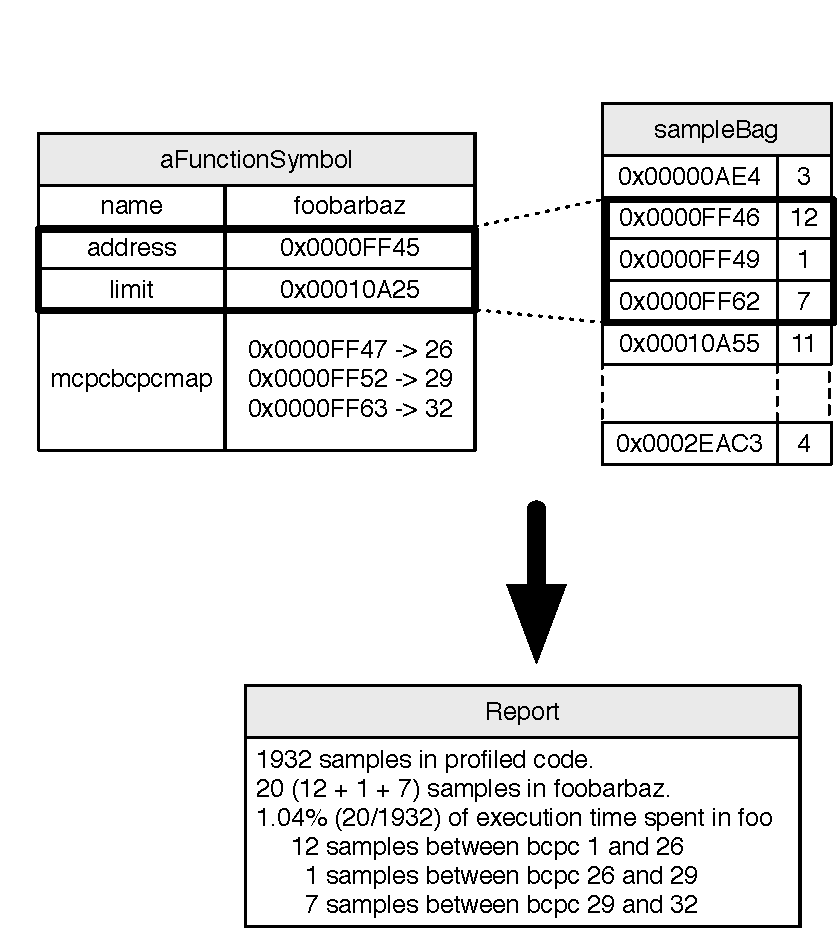
\includegraphics[width=1.0\linewidth]{NewMapping}
         \caption{Mapping with new feature}
         \figlabel{fig:NewMapping}
     \end{center}
 \end{figure}
 
%: % % % % % % % % % % % % % % % % % % % % % % % % % % % % % % % % %

\section{Example}

Intro: this is a concrete example on a benchmark. (tinyBench ?)

montrer avant / apres.



\figref{fig:Example} describes bla.

\begin{figure}
    \begin{center}
		\noindent \begin{tabular}{l | l}
		Existing profiler report & Accurate profiler report \\		
		\midrule
		rapport 1 & rapport 2 \\	
		\end{tabular}
	\caption{Example of profiling reports}
    \label{fig:Example}
    \end{center}
\end{figure}


%: % % % % % % % % % % % % % % % % % % % % % % % % % % % % % % % % %
\section{Related Work}\seclabel{relatedWork}

intro 

\subsection{Smalltalk profilers}

*profiling in Pharo-Smalltalk
In Squeak, 2 (?) profiling tools are available in the image: MessageTally and VM profiler. Both are sampling profilers, but they are not used for the same purpose. MessageTally = image side, VM profiler = vm side.

*messageTally [reference]
description, comparison
*spy [reference]
description, comparison
*gadgetProfiler [reference]
description, comparison

\subsection{Other VM profilers}

jvisualvm

%: % % % % % % % % % % % % % % % % % % % % % % % % % % % % % % % % %
\section{Conclusion and Future Work}\seclabel{conclusion}

Future work: UI, Windows. -> engineering.

% windows
% UI

%{\footnotesize \myparagraph{Acknowledgments} We thank 
%Oscar Nierstrasz, 
%Lukas Renggli,
%Eric Tanter, and 
%Renato Cerro 
%for their comments on an early draft of this paper. We also thank Aleksandar Prokopec for his help with Scala collections.}
%: % % % % % % % % % % % % % % % % % % % % % % % % % % % % % % % % %

%{\small
\bibliographystyle{elsarticle-num}
\bibliography{sista}
%\bibliography{hapao}
%}


%\appendix 
\end{document}

